\section{Materiales y métodos}\label{sec:metodos}
\subsection{Caso sintético y datos}
El caso es sintético y no representa una obra ni un levantamiento reales. Se adopta $Q_0=12.00\,\Qs$, $g=9.81\,\mathrm{m/s^2}$ y $z_J=100.00$ m. Los anchos de fondo son $b_0=4$ m (canal principal), $b_1=3$ m y $b_2=2$ m; la Tabla~\ref{tab:datos} reúne el resto. El canal principal no interviene en las ecuaciones 1D, pero sí en la geometría 2D. Se consideran cinco ángulos entre ejes: $30^\circ$, $45^\circ$, $60^\circ$, $90^\circ$ y $120^\circ$. El esquema isométrico del canal se muestra en la Figura~\ref{fig:esquema}. Los datos están en \path{datos/datos_entrada.json}.

\begin{table}[H]
\centering\small
\caption{Datos de entrada del caso nominal.}\label{tab:datos}
\begin{tabular}{lrr}
\toprule
Parámetro & Ramal 1 & Ramal 2\\\midrule
Ancho de fondo $b$ (m) & 3.00 & 2.00\\
Longitud $L$ (m) & 200 & 150\\
Rugosidad de Manning $n$ & 0.015 & 0.018\\
Pendiente de fondo $S$ (m/m) & 0.0008 & 0.0010\\
Calado de control $y_d$ (m) & 1.60 & 1.40\\
Cota de fondo en la unión $z_J$ (m) & 100.00 & 100.00\\
Coeficiente local $K$ & 0.20 & 0.20\\\bottomrule
\end{tabular}
\Fuente{Elaboración propia (caso sintético).}
\end{table}

\begin{figure}[H]
\centering
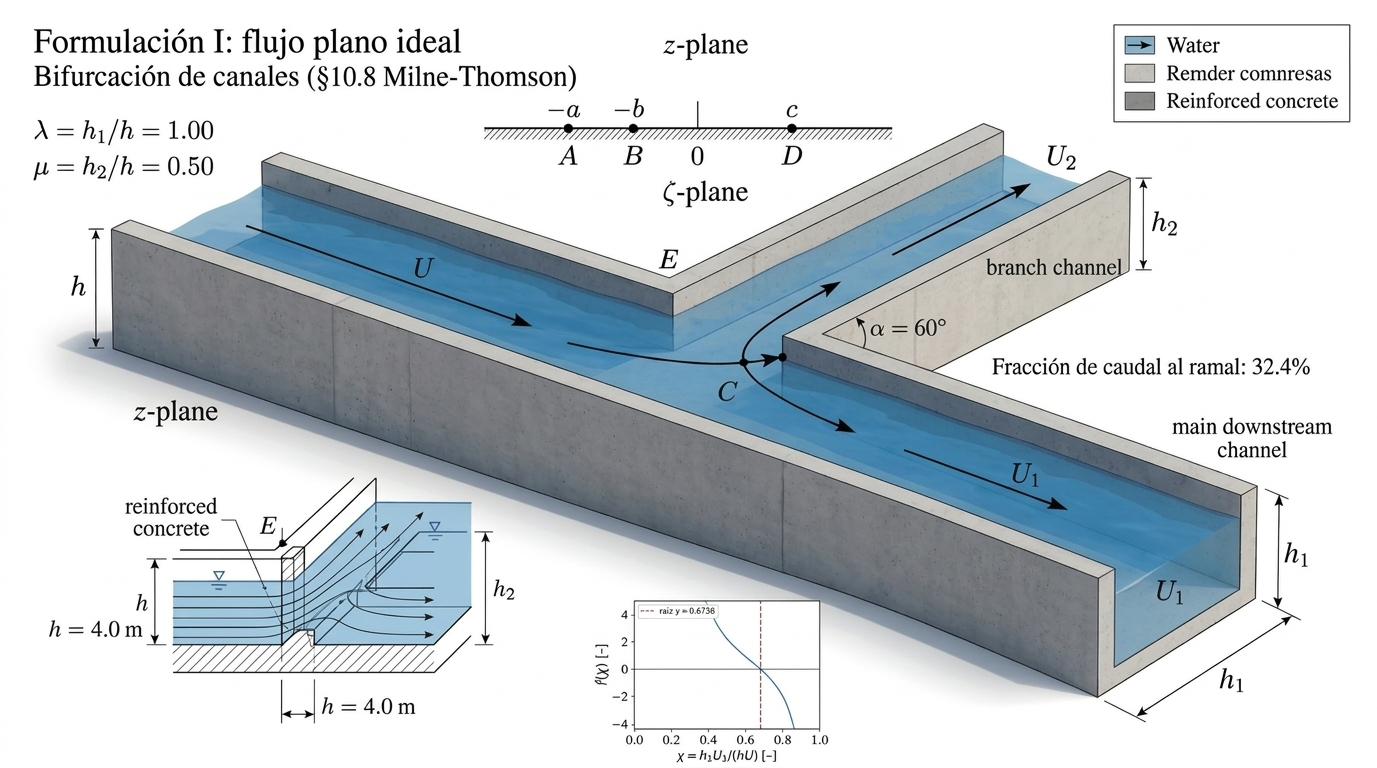
\includegraphics[width=0.82\linewidth,height=0.42\textheight,keepaspectratio]{2.png}
\caption{Esquema isométrico del canal bifurcado y nomenclatura. Ilustrativo, no a escala.}\label{fig:esquema}
\Fuente{Elaboración propia.}
\end{figure}

\subsection{Implementación numérica y reproducibilidad}
El código está en Python 3.13 con NumPy 2.5, pandas 3.0 y Matplotlib 3.11. La Formulación I se resuelve con Newton--Raphson sobre \eqref{eq:f1} para cada $\alpha$. La Formulación II usa Newton amortiguado con el jacobiano analítico \eqref{eq:sistema}, resolución del sistema lineal con \texttt{numpy.linalg.solve}, tolerancia $10^{-12}$ sobre $\|\mathbf F\|_\infty$, máximo de 50 iteraciones y retroceso hasta un factor mínimo de $10^{-4}$. El punto inicial reparte $Q_0$ según las conductancias de los ramales evaluadas con sus calados de control y coloca $H_J$ $0.05$ m sobre el mayor nivel terminal. El Monte Carlo usa 1500 realizaciones, desviaciones independientes y normales (caudal 5\pc, anchos 2\pc, Manning 10\pc, longitudes 2\pc, pendientes 5\pc, calados de control 0.04 m, $K$ 0.10 en valor absoluto) y la semilla fija \texttt{20261103}. Los resultados 1D se regeneran con \path{codigo/newton_bifurcacion.py}, que imprime las versiones de las bibliotecas y el historial de iteraciones.

\subsection{Pruebas de verificación del código}
Se aplican tres pruebas: (i) simetría analítica, con dos ramales idénticos el reparto debe ser $Q_0/2$ a cada lado; (ii) conservación de masa del caso nominal, $Q_1+Q_2-Q_0$; y (iii) contraste con una red de ocho canales publicada \citep[cap.~6]{chaudhry2008}. Además, las hojas de resultados 1D entregadas junto con el libro de HEC-RAS se contrastan con las soluciones recalculadas.

\subsection{Modelo bidimensional}\label{sec:hecras}
Las simulaciones se ejecutaron en HEC-RAS 7.0.1 (junio de 2026, unidades SI) por un integrante del grupo; los proyectos de $45^\circ$ y $90^\circ$ están disponibles, y para $30^\circ$, $60^\circ$ y $120^\circ$ solo se dispone de los resultados (CSV y libro). Los archivos del proyecto muestran lo siguiente.
\begin{itemize}
\item \textbf{Malla:} una sola malla por ángulo, de tamaño medio de celda 0.46 m (6372 celdas, $45^\circ$) y 0.53 m (4839 celdas, $90^\circ$). No hay refinamientos sistemáticos, por lo que no se evalúa independencia de malla.
\item \textbf{Ecuaciones:} onda difusiva (\textit{Diffusion Wave}), $\theta=1$, sin formulación de turbulencia (Sección~\ref{sec:dw}).
\item \textbf{Rugosidad:} Manning base 0.018, con zonas de 0.015 (ramal 1) y 0.018 (ramal 2) en la configuración prevista; la configuración efectivamente simulada se reconstruye en la Sección~\ref{sec:config}.
\item \textbf{Condiciones de borde:} hidrograma triangular de entrada con pico de $12\,\Qs$ hacia el minuto 112, base de unos 180 min y volumen $64\,800\ \mathrm{m^3}$; salidas con pendiente de fricción (calado normal) de 0.0008 (ramal 1) y 0.0010 (ramal 2), no con cota fija.
\item \textbf{Tiempo:} simulación de 3 h 18 min, salida cada 2 min y paso de cálculo de 10 s ($45^\circ$) y de 2 s ($90^\circ$).
\end{itemize}
\begin{table}[H]
\centering\small
\caption{Parámetros de los planos HEC-RAS disponibles.}\label{tab:planes}
\begin{tabular}{lcc}
\toprule
Parámetro & $45^\circ$ (\texttt{HEC\_RAS\_FSL.p02}) & $90^\circ$ (\texttt{Modelo90g.p01})\\\midrule
Versión de HEC-RAS & 7.0.1 (junio de 2026) & 7.0.1 (junio de 2026)\\
Conjunto de ecuaciones 2D & Onda difusiva & Onda difusiva\\
Número de celdas & 6372 & 4839\\
Tamaño medio de celda (m) & 0.46 & 0.53\\
Paso de cálculo (s) & 10 & 2\\
Intervalo de salida & 2 min & 2 min\\
Ventana de simulación & 3 h 18 min & 3 h 18 min\\
Tolerancia de nivel del agua (m) & 0.003 & 0.01\\
Error de balance de volumen (\%) & $1.2\times10^{-6}$ & $6.3\times10^{-5}$\\\bottomrule
\end{tabular}
\Fuente{Archivos HDF de los planos (\path{Plan Data/Plan Parameters} y \textit{Volume Accounting}).}
\end{table}

Los caudales por sección se calculan como suma de $d\,v\,\Delta s$ en perfiles transversales extraídos de los \emph{rásteres} de calado y velocidad \emph{máximos} \citep{hecmanual}, con el cuaderno \path{codigo/Codigo_Calculo_de_Datos_de_salida_Python.ipynb}. Los máximos por celda no son simultáneos en el tiempo; el hidrograma es lento (una variación de unos $0.2\,\Qs$ por minuto), por lo que se asume un estado cuasipermanente en el pico, supuesto que no se verificó con las series temporales. La incertidumbre de medición del reparto en el 2D se toma como la máxima diferencia entre dos productos de caudal (libro de resultados y suma de los CSV): $U_{2D}=0.0078$.

\subsection{Criterios de aceptación y de sesgo}\label{sec:criterios}
Se fijaron antes de inspeccionar el sesgo: error del caudal del ramal $\varepsilon(Q_2)\leq10\pc$ es aceptable y $\leq20\pc$ marginal; diferencia de nivel en la unión $|\Delta y_J|\leq0.10$ m aceptable y $\leq0.20$ m marginal. Son criterios operativos propuestos por el grupo y pendientes de confirmación por el docente. Se comparan cuatro predictores: Formulación I; Formulación II con datos nominales; Formulación II con la configuración efectivamente simulada (rugosidad, pendientes y calados reales del 2D); y Formulación II con calado normal en las salidas, que no usa dato alguno del 2D. La comparación justa es contra la configuración simulada, porque la nominal no coincide con la del 2D.

\subsection{Balance de masa}
El balance de masa global se tomó del resumen de volúmenes de cada plan (\textit{Volume Accounting}; \citealt{hecmass}), y se contrastó con la hoja \path{Balance de masa.xlsx}. El error relativo se define como $100\,(V_\mathrm{ent}-V_\mathrm{sal}-\Delta V_\mathrm{alm})/V_\mathrm{ent}$.
